\graphicspath{{weeks/images/week_4/}}

Test CI

\textcolor{red}{ATTENTION : problème de projection - carte d'erreur FEM}

\subsection{Reproduction résultats - Article 2104.08426}

Dans un premier temps, j'ai cherché à implémenter en Python les deux méthodes présentées dans l'article 2104.08426, permettant de calculer une ADF ("Approach Distance Function"). On retrouve le calcul d'une ADF sur un polygone qui représente le bord d'une ellipse par les deux méthodes suivantes :  la méthode REQ (R-equivalence) dans la Figure \ref{REQ} et la méthode MVP ("Mean Value Potential") dans la Figure \ref{MVP}.

\begin{minipage}{0.38\linewidth}
	\begin{figure}[H]
		\centering
		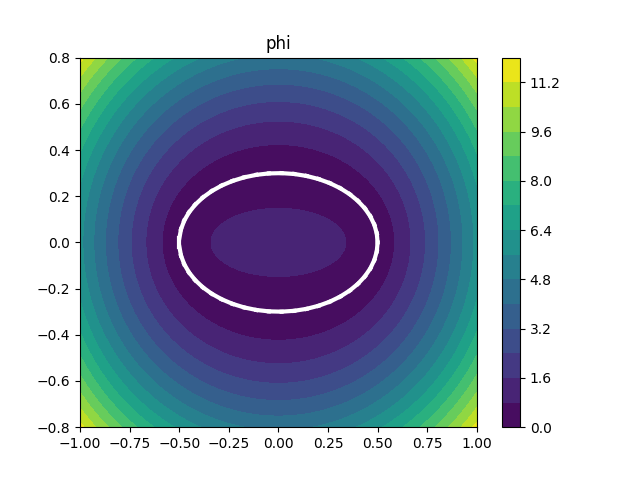
\includegraphics[width=0.7\linewidth]{"article/REQ_ellipse.png"}
		\caption{ADF par REQ sur une ellipse.}
		\label{REQ}
	\end{figure}
\end{minipage}
\begin{minipage}{0.58\linewidth}
	\begin{figure}[H]
		\centering
		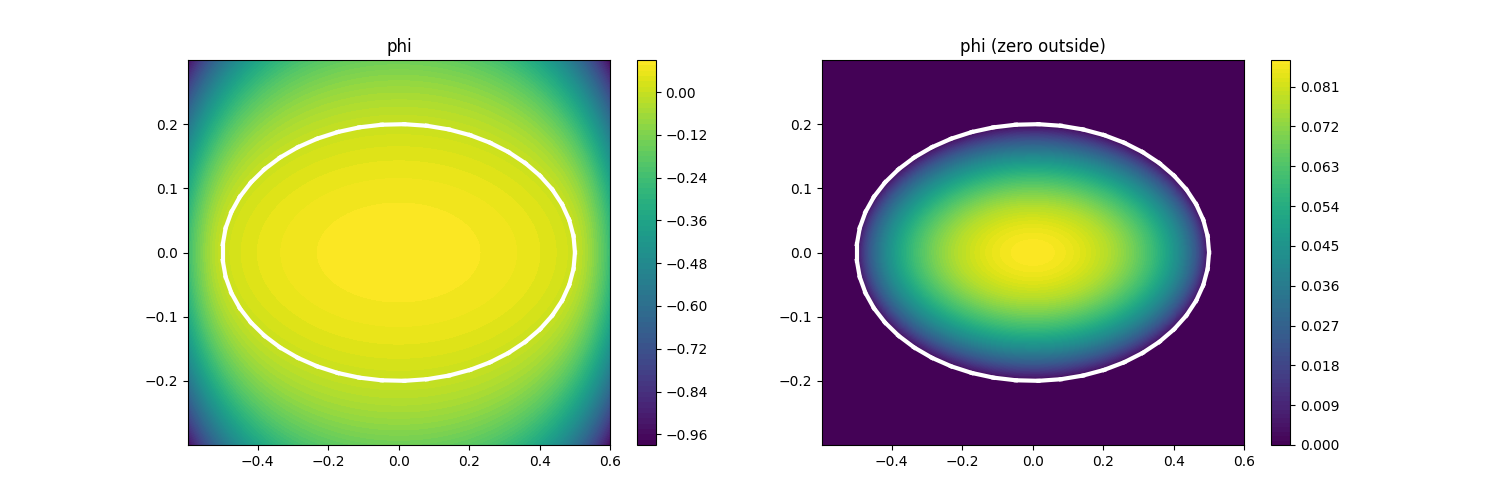
\includegraphics[width=\linewidth]{"article/MVP_ellipse.png"}
		\caption{ADF par MVP sur une ellipse.}
		\label{MVP}
	\end{figure}
\end{minipage}

\subsection{Entraînement du PINNs à apprendre une solution unique}

\subsubsection{Problème considéré}

\textbf{EDP :} On considère le problème de Poisson avec condition de Dirichlet homogène ($g=0$), définie par

Trouver $u : \Omega \rightarrow \mathbb{R}^d (d=1,2,3)$ tel que
\begin{equation}
	\left\{
	\begin{aligned}
		-\Delta u &= f, \; &&\text{dans } \; \Omega, \\
		u&=g, \; &&\text{sur } \; \partial\Omega,
	\end{aligned}
	\right. \tag{$\mathcal{P}$} \label{pb_initial}
\end{equation}
avec $\Delta$ l'opérateur de Laplace.

\textbf{Géométrie :} On considère $\Omega$ comme étant un cercle de rayon $r$ et de centre $(x_0,y_0)$. 

Pour simplifier, on va considérer que $\Omega$ est entièrement contenu dans un carré $\mathcal{O}$ (Figure \ref{geom_circle}). 

\begin{minipage}{0.38\linewidth}
	\begin{figure}[H]
		\centering
		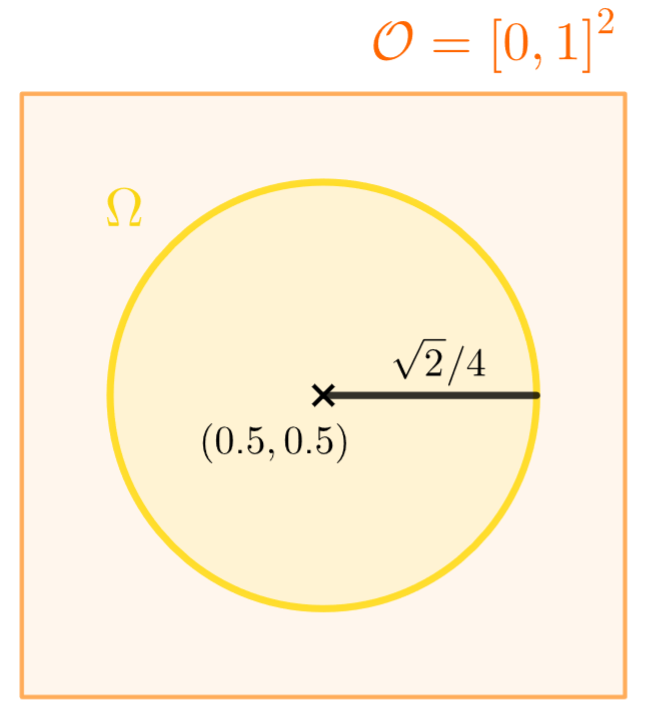
\includegraphics[width=0.7\linewidth]{"training/geom_circle.png"}
		\caption{Domaine considéré.}
		\label{geom_circle}
	\end{figure}
\end{minipage}
\begin{minipage}{0.68\linewidth}
	On considère la solution analytique $u_{ex}$, définie par
	\begin{equation*}
		u_{ex}(x,y)=S\times\sin\left(\frac{1}{r^2}\pi((x-x_0)^2+(y-y_0)^2)\right)
	\end{equation*}
	
	Ce qui nous fournit le terme source $f$, définie par
	\begin{align*}
		f(x,y)=\frac{4}{r^4}\pi^2&S((x-x_0)^2+(y-y_0)^2)\sin\left(\frac{1}{r^2}\pi((x-x_0)^2+(y-y_0)^2)\right) \\
		&-\frac{4}{r^2}\pi S \cos\left(\frac{1}{r^2}\pi((x-x_0)^2+(y-y_0)^2)\right)
	\end{align*}
\end{minipage}
\begin{Rem}
	On voit que sur le cercle, le problème est bien homogène.
	
	De plus, on notera qu'un choix simple peut être de prendre le carré $[x_0-r-\epsilon,x_0+r+\epsilon]\times[y_0-r-\epsilon,y_0+r+\epsilon]$ où $\epsilon>0$ est un paramètre fixé dans le but que $\Omega$ soit entièrement compris dans $\mathcal{O}$.
\end{Rem}

\subsubsection{Entraînement du PINNs}

On fixe $r=\sqrt{2}/4$, $(x_0,y_0)=(0.5,0.5)$ et $S=0.5$ et on considère ici que l'on souhaite entraîner un PINNs à apprendre cette solution. On utilisera l'implémentation développé dans le module ScimBA\footnote{\url{https://sciml.gitlabpages.inria.fr/scimba/}}. 

On notera que l'article 2104.08426 présente comment imposer les conditions au bord de manière exacte. C'est pourquoi, on considérera deux cas :
\begin{enumerate}[label=\textbullet]
	\item on apprend directement la solution $u$. La loss totale regroupe alors la loss sur le résidu et la loss sur le bord.
	\item on apprend $w$ tel que $u=\phi w$ avec $\phi$ notre fonction levelset. La loss ne contient alors que la loss sur le résidu. 
\end{enumerate}
Ainsi, une première étape a été de rajouter, dans l'implémentation de ScimBa, la possibilité de définir un domaine à partir d'une fonction levelset. Ainsi pour obtenir un sampling de points à l'intérieur de $\Omega$, il suffit de générer un échantillon de point sur le carré $\mathcal{O}$ et de ne garder que les points tels que $\phi(x,y)<0$. Pour générer un échantillon de point sur le bord du domaine $\Omega$, on a fait le choix pour l'instant de prendre les points tels que $|\phi(x,y)|<\epsilon$ avec $\epsilon=1e-5$ (Figure \ref{sampling_0}).

\begin{figure}[H]
	\centering
	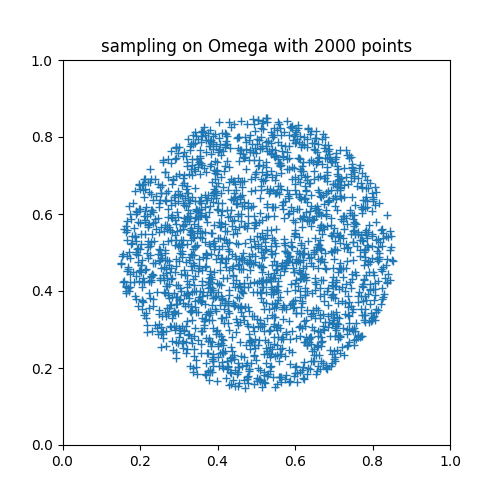
\includegraphics[width=0.5\linewidth]{"training/sampling_0.png"}
	\caption{Sampling à l'intérieur et au bord du cercle considéré.}
	\label{sampling_0}
\end{figure}

\begin{Rem}
	Pour le sampling du bord, c'est un choix qui ne sera pas conserver, il faudra trouver une solution plus rapide-précise que celle-ci.
\end{Rem}

On peut alors entraîner le PINNs à apprendre notre solution. On choisira la configuration suivante :
\begin{figure}[H]
	\centering
	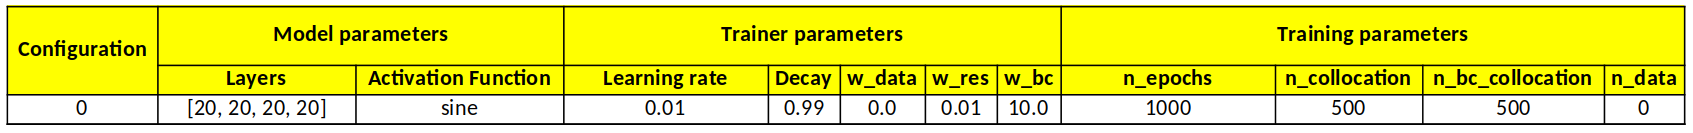
\includegraphics[width=\linewidth]{"training/config_0.png"}
	\caption{Paramètres d'entraînement considéré pour le PINNs.}
	\label{config_0}
\end{figure}

On va alors entraîner un modèle à apprendre $u$ (Figure \ref{model_0}) et un autre à apprendre $w$ (Figure \ref{model_0_exact_bc}) avec ces mêmes paramètres dans le but de comparer les résultats.

\begin{minipage}{0.48\linewidth}
	\begin{figure}[H]
		\centering
		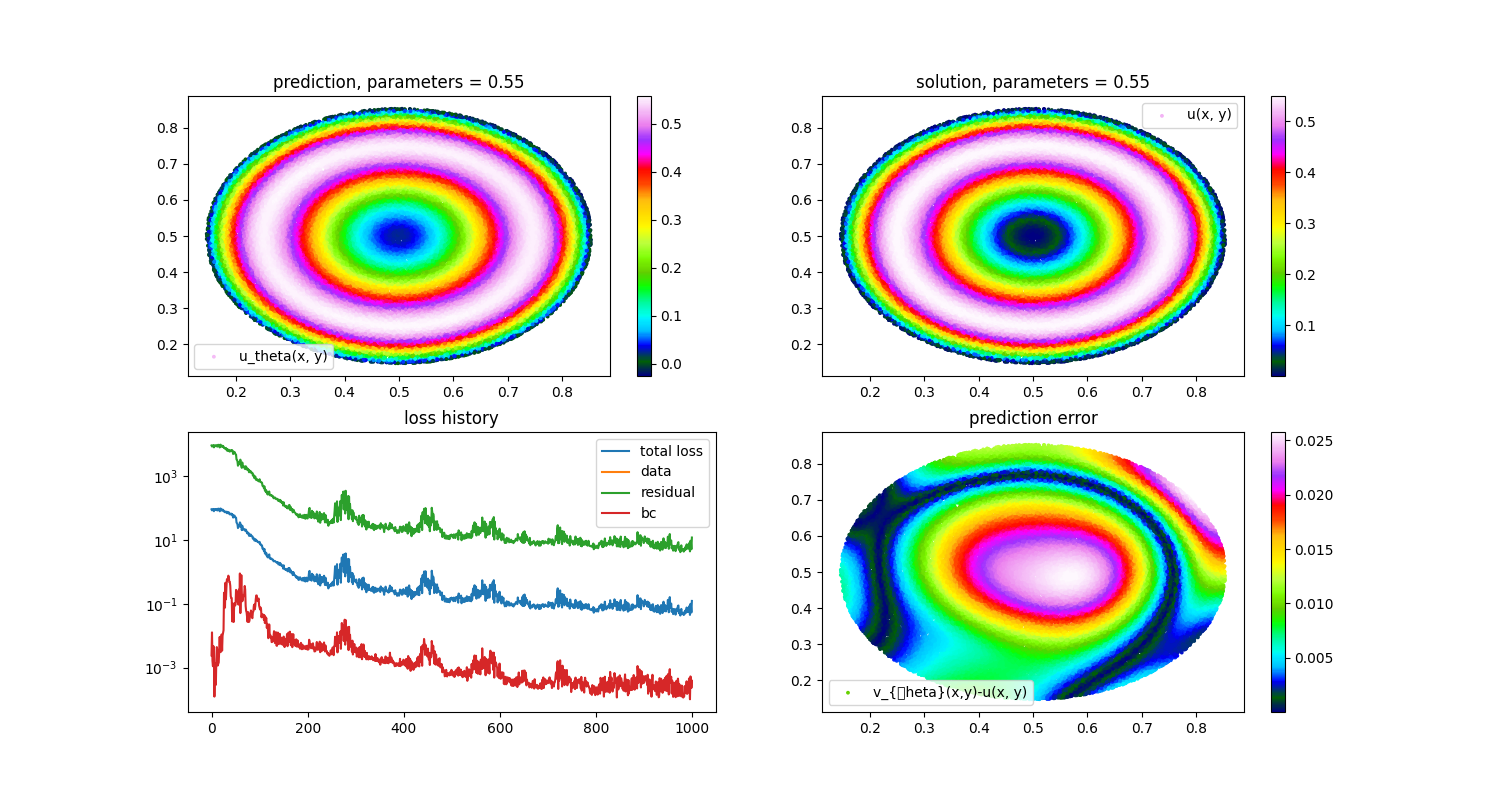
\includegraphics[width=\linewidth]{"training/model_0.png"}
		\caption{Fin d'entraînement - Modèle sur $u$.}
		\label{model_0}
	\end{figure}
\end{minipage}
\begin{minipage}{0.48\linewidth}
	\begin{figure}[H]
		\centering
		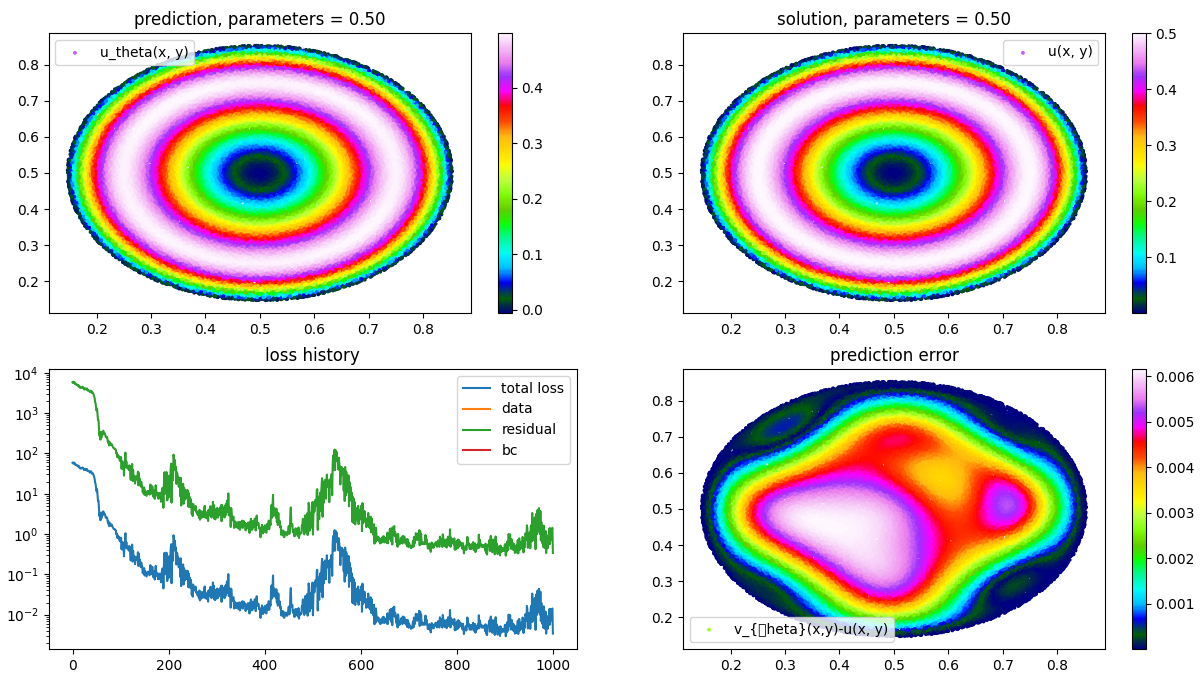
\includegraphics[width=\linewidth]{"training/model_0_exact_bc.png"}
		\caption{Fin d'entraînement - Modèle sur $w$.}
		\label{model_0_exact_bc}
	\end{figure}
\end{minipage}

\begin{Rem}
	Il semblerait que le modèle sur $w$ soit 10 fois plus précis en terme d'erreur.
	
	De plus, on remarque bien, sur la carte d'erreur, sur le modèle sur $u$ a des erreurs au bord, ce qui risque de poser problème dans la correction. 
\end{Rem}

\subsubsection{Correction sur les prédictions du PINNs}

On note $\tilde{\phi}$ la prédiction d'un des PINNs précédent. On ne va considérer ici que la correction par addition, on pose alors
\begin{equation*}
	\tilde{u}=\tilde{\phi}+\tilde{C}
\end{equation*}
et on cherche à trouver $\tilde{C}: \Omega \rightarrow \mathbb{R}^d$ solution du problème
\begin{equation*}
	\left\{\begin{aligned}
		-\Delta \tilde{u}&=f, \; &&\text{on } \Omega, \\
		\tilde{u}&=g, \; &&\text{in } \Gamma.
	\end{aligned}\right.
\end{equation*}
avec $g=0$ dans le cas considéré.
On cherche alors à trouver $\tilde{C}: \Omega \rightarrow \mathbb{R}^d$ solution du problème
\begin{equation*}
	\left\{\begin{aligned}
		-\Delta \tilde{C}&=\tilde{f}, \; &&\text{on } \Omega, \\
		\tilde{C}&=0, \; &&\text{in } \Gamma.
	\end{aligned}\right. %\tag{$\mathcal{C}_{+}$}
\end{equation*}
avec $\tilde{f}=f+\Delta\tilde{\phi}$.

On cherche alors à tester la correction sur les deux modèles précédents (celui où on apprend $u$ et celui où on apprend $w$). On testera l'utilisation de FEM et de $\phi$-FEM dans les deux cas.

\textbf{Résultats avec le modèle sur $u$ :}

\begin{minipage}{0.48\linewidth}
	\begin{figure}[H]
		\centering
		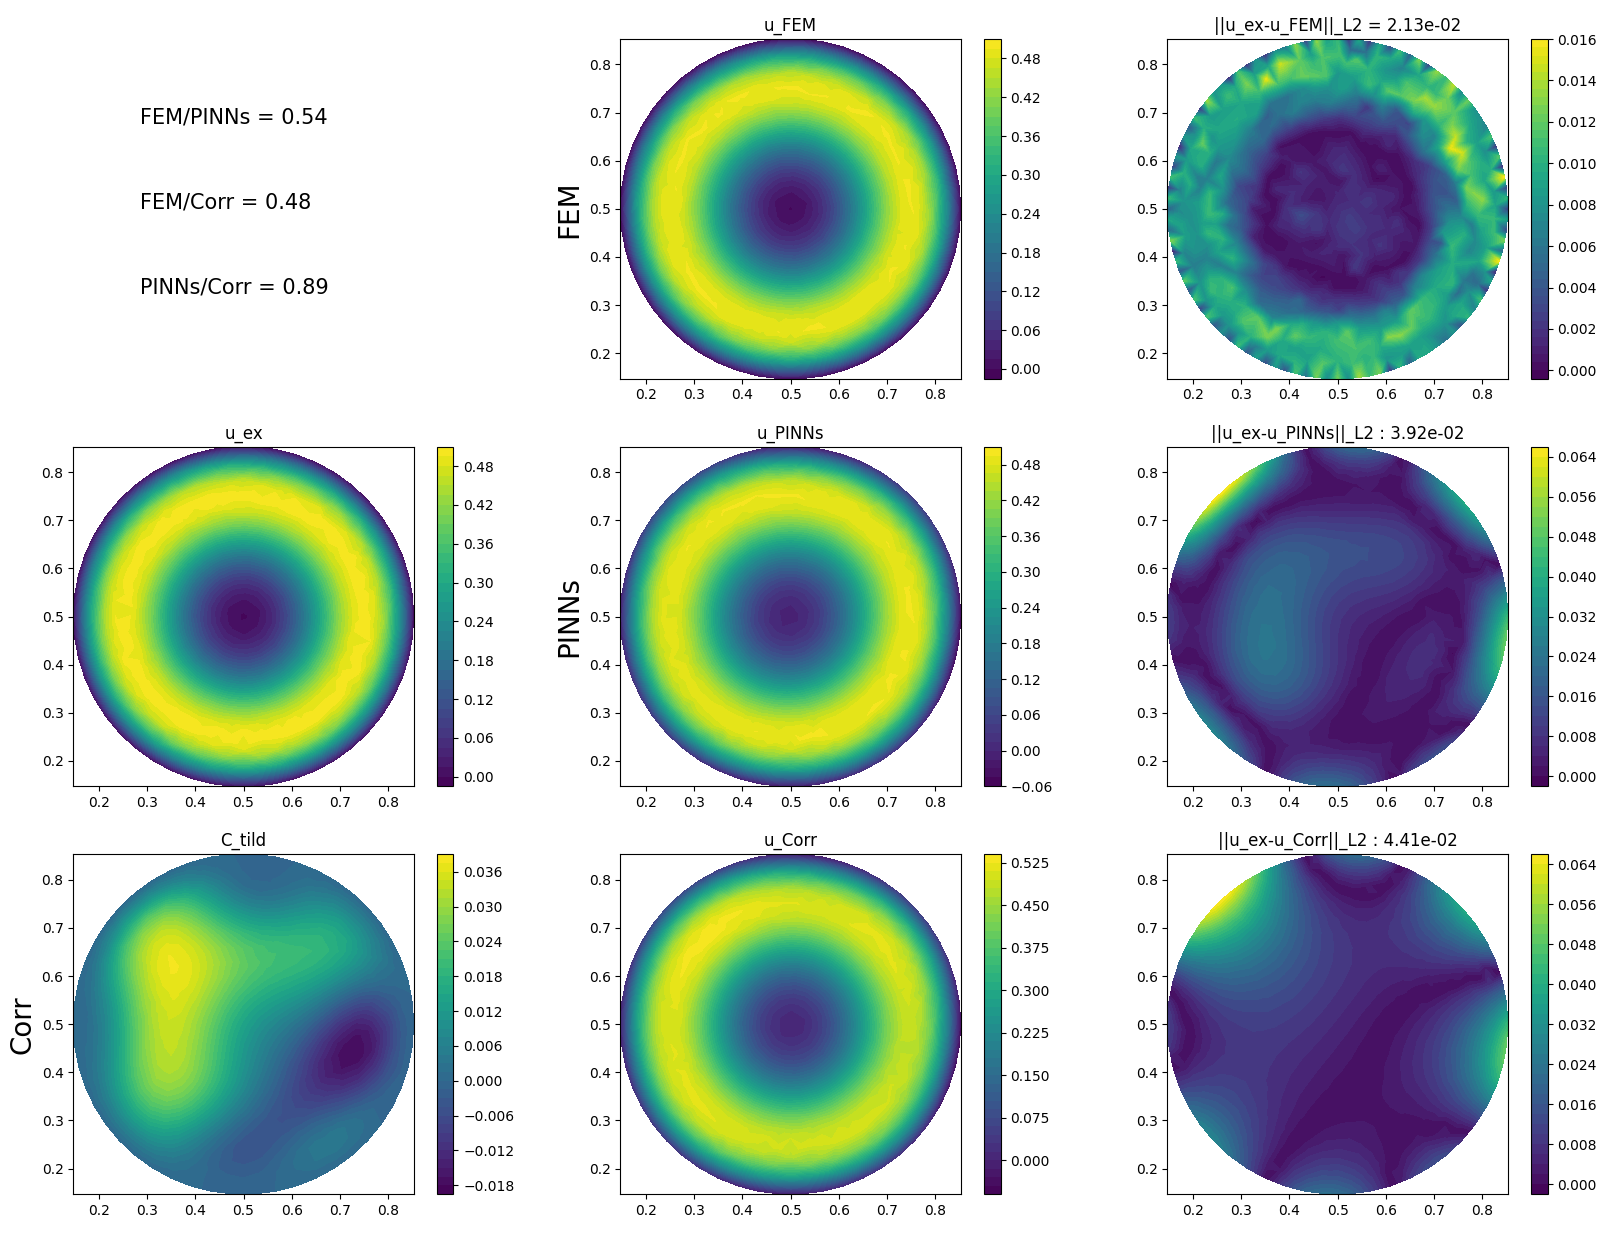
\includegraphics[width=\linewidth]{"corr/corr_fem_0.png"}
		\caption{Correction avec FEM - Modèle sur $u$.}
		\label{corr_fem_0}
	\end{figure}
\end{minipage}
\begin{minipage}{0.48\linewidth}
	\begin{figure}[H]
		\centering
		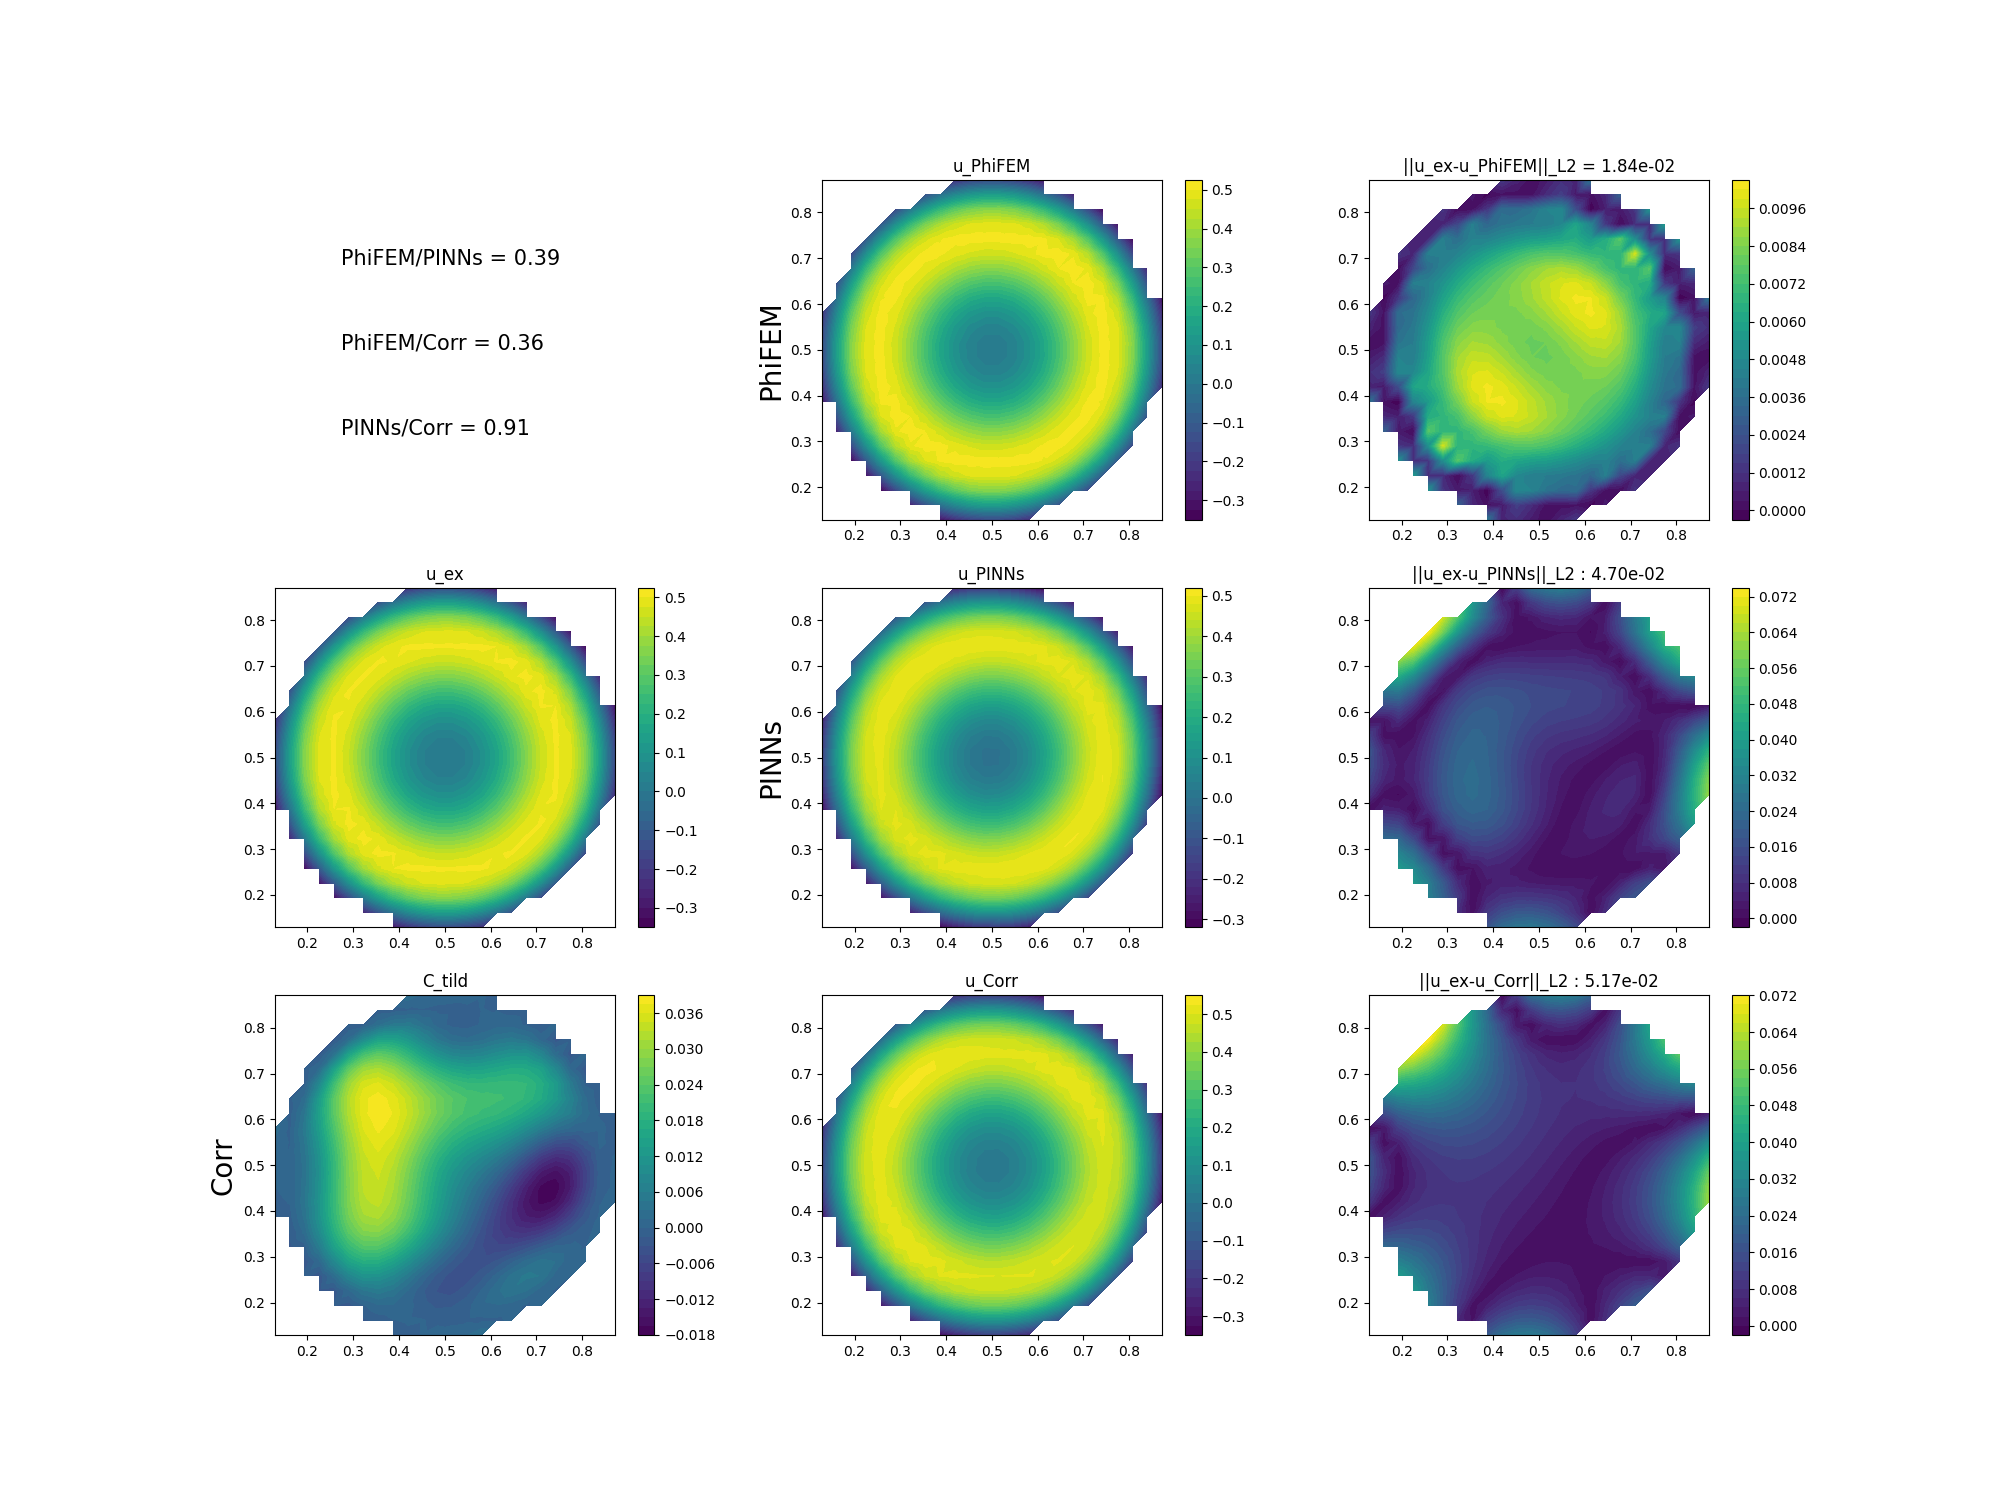
\includegraphics[width=\linewidth]{"corr/corr_phifem_0.png"}
		\caption{Correction avec $\phi$-FEM - Modèle sur $u$.}
		\label{corr_phifem_0}
	\end{figure}
\end{minipage}

\textbf{Résultats avec le modèle sur $w$ :}

\begin{minipage}{0.48\linewidth}
	\begin{figure}[H]
		\centering
		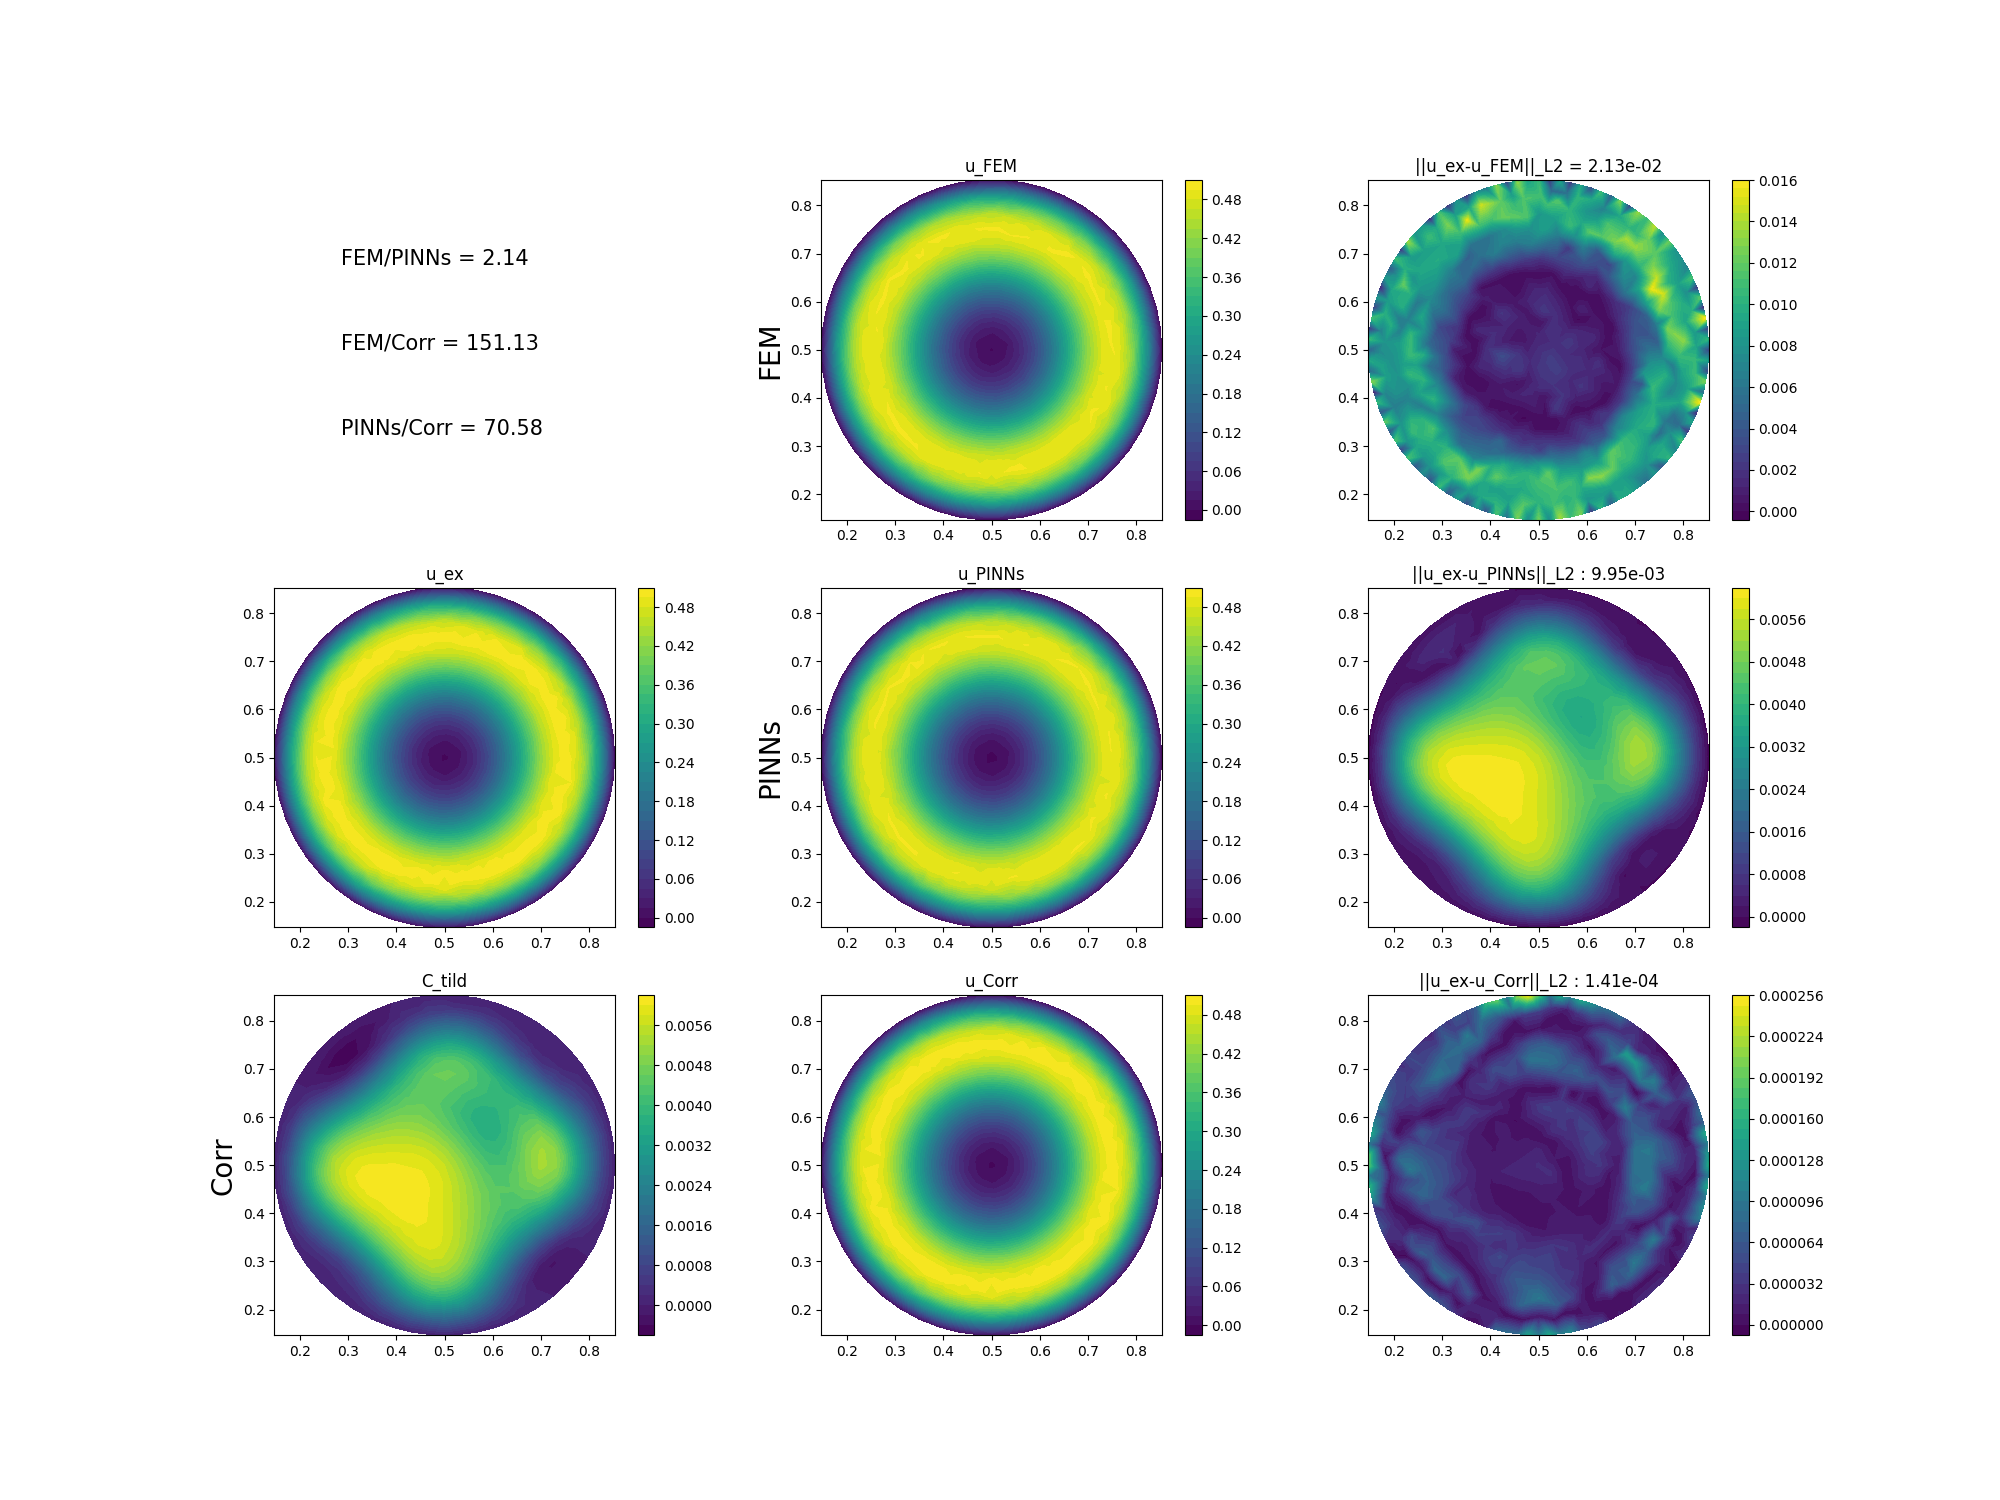
\includegraphics[width=\linewidth]{"corr/corr_fem_0_exact_bc.png"}
		\caption{Correction avec FEM - Modèle sur $w$.}
		\label{corr_fem_0_exact_bc}
	\end{figure}
\end{minipage}
\begin{minipage}{0.48\linewidth}
	\begin{figure}[H]
		\centering
		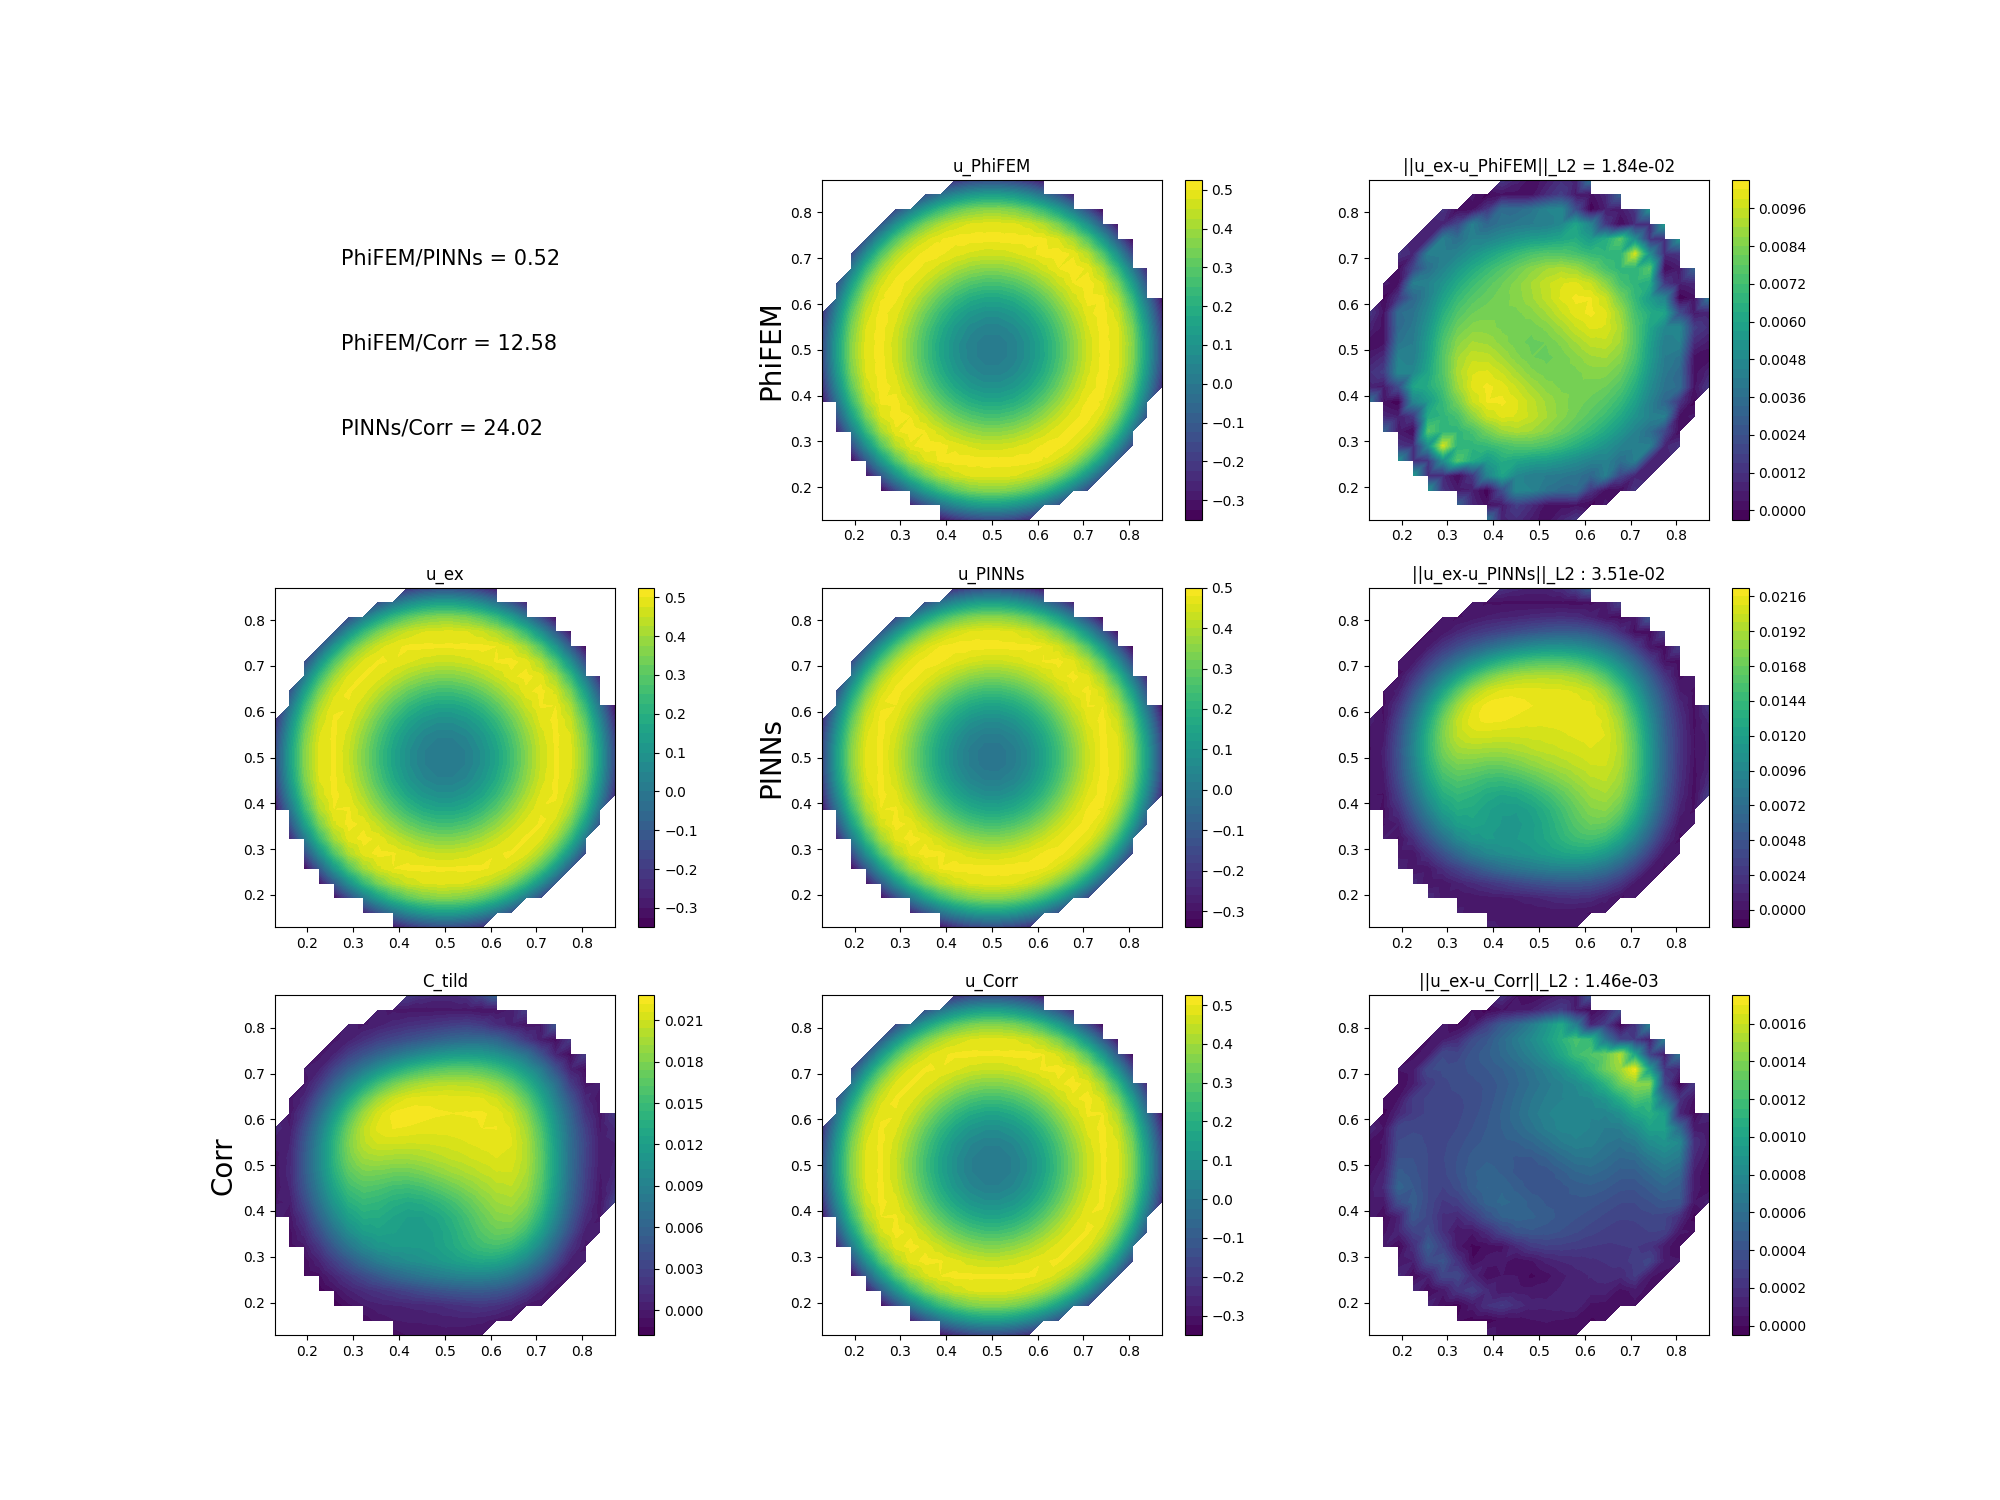
\includegraphics[width=\linewidth]{"corr/corr_phifem_0_exact_bc.png"}
		\caption{Correction avec $\phi$-FEM - Modèle sur $w$.}
		\label{corr_phifem_0_exact_bc}
	\end{figure}
\end{minipage}